\documentclass{magnolia}

\magtex{tex_driver={pdftex},
        tex_packages={siunitx}}
\magfiche{document_nom={Récursivité, horizon},
          auteur_nom={François Fayard},
          auteur_mail={francois.fayard@auxlazaristeslasalle.fr}}
\magcours{cours_matiere={maths},
          cours_niveau={mpsi},
          cours_chapitre_numero={1},
          cours_chapitre={Ligne d'horizon}}
\magmisenpage{}
\maglieudiff{}
\magprocess

\begin{document}
%BEGIN_BOOK


\section{Ligne d'horizon}

Le problème de la ligne d'horizon est le suivant~: étant donnés un certain nombre de rectangles posés sur
l'axe des abscisses, quelle sera la ligne d'horizon visible. Les rectangles seront représentés par des
tuples \verb!(a, b, h)! où $a$ est l'abscisse du coin inférieur gauche, $b$ est l'abscisse du coin
inférieur droit et $h$ la hauteur du bâtiment. La liste des bâtiments nous sera donc donnée par une
liste de type \verb!list[tuple[int, int, int]]!. Par exemple, la figure 1, représente les bâtiments donnés
par la liste \verb!bat = [(0, 5, 3), (1, 3, 2), (2, 4, 4), (6, 7, 2)]!.
\begin{center}
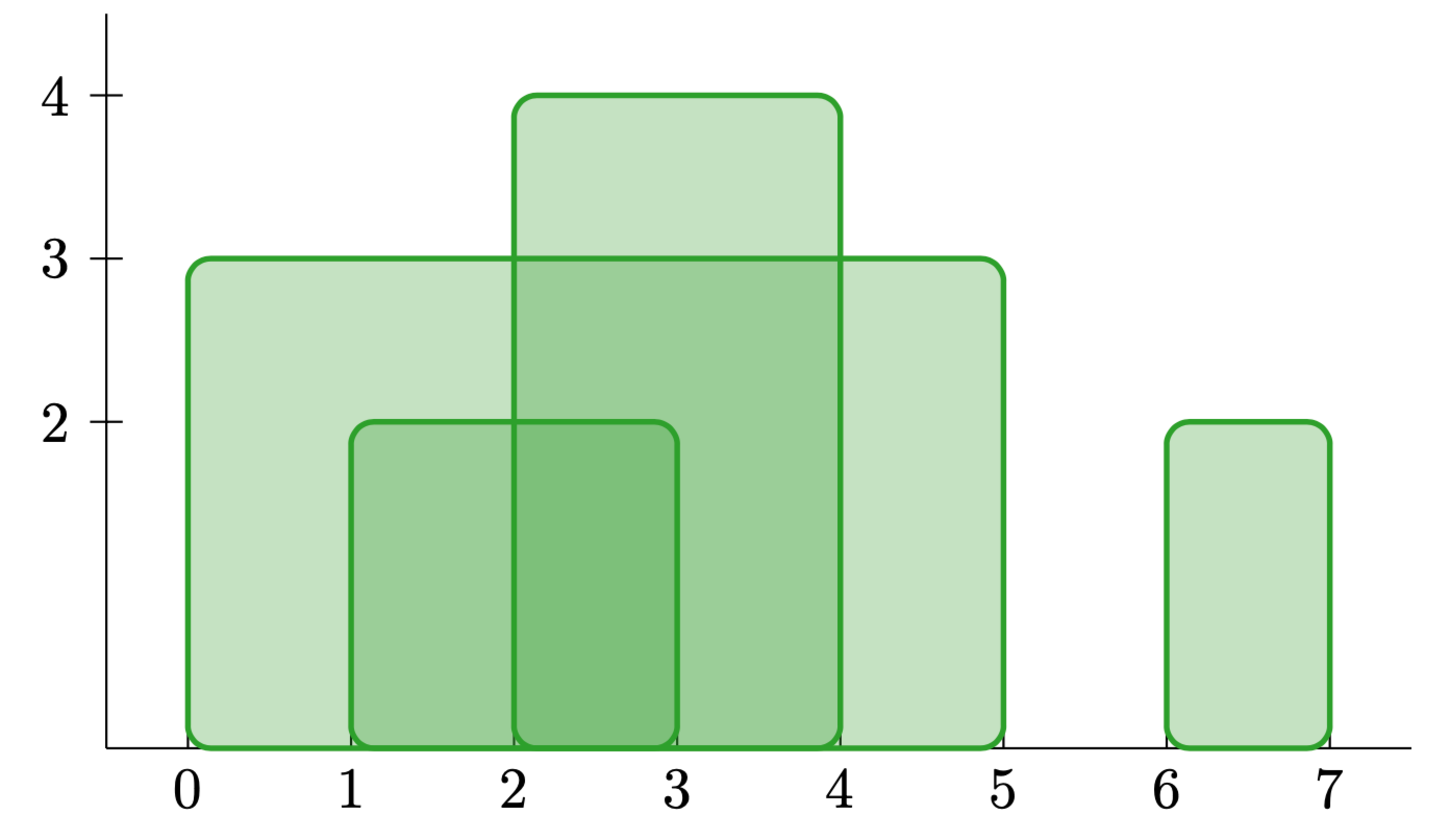
\includegraphics[width=0.5\textwidth]{../../Commun/Images/python-tp-horizon-1}\\
\textsc{Figure 1}
\end{center}
La ligne d'horizon est quant à elle donnée par la liste des points à chaque changement d'ordonnée~: on donne
l'abscisse et l'ordonnée à droite du changement. Dans notre exemple, la ligne d'horizon visualisée sur
la figure 2 sera représentée par \verb!hor = [(0, 3), (2, 4), (4, 3), (5, 0), (6, 2), (7, 0)]!.
\begin{center}
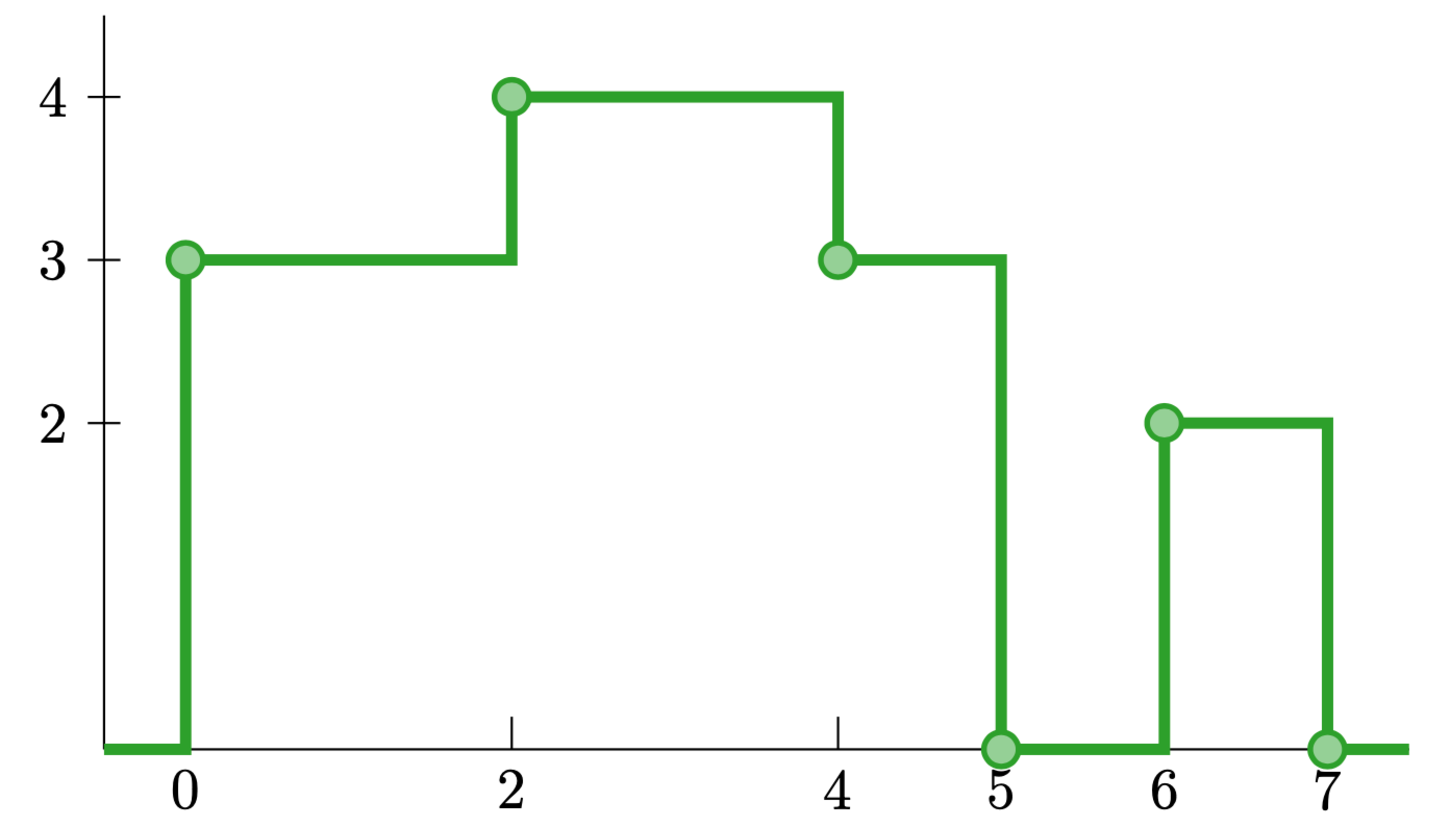
\includegraphics[width=0.5\textwidth]{../../Commun/Images/python-tp-horizon-2}\\
\textsc{Figure 2}
\end{center}
\begin{questions}
\question Si \verb!hor! est une ligne d'horizon, que peut-on dire de \verb!hor[-1][1]!~?
\end{questions}

\subsection{Un cas simple}

Dans cette partie, on suppose que les abscisses des bords des rectangles sont des entiers compris entre
0 et $n-1$.
\begin{questions}
\question Écrire une fonction \verb!hauteurs(bat: list[tuple[int, int, int]], n: int) -> list[int]! qui prend
  en argument une liste de rectangles et leur abscisse maximale, et renvoie la liste \verb!h! des hauteurs de la
  ligne d'horizon~: pour tout $i\in\intere{0}{n-1}$, \verb!h[i]! est la hauteur de la ligne d'horizon
  juste à droite du point d'abscisse $i$. Avec l'exemple ci-dessus, cette fonction appelée avec $n=8$ nous
  renverrait la liste \verb![3, 3, 4, 4, 3, 0, 2, 0]!.
\question En utilisant ce qui précède, écrire une fonction
\begin{center}
  \verb!horizon_entier(bat: list[tuple[int, int, int]], int: n) -> list[tuple[int, int]]!
\end{center}
qui renvoie la liste des points de la ligne d'horizon.
\question Exprimer la complexité de ce calcul en fonction de paramètres de votre choix.
\end{questions}

\subsection{Le cas général}

On ne fait cette fois-ci plus aucune hypothèse sur les abscisses des rectangles. Nous supposerons par contre
pour simplifier que les abscisses des bords des rectangles sont toujours distinctes.
\begin{questions}
\question Écrire une fonction \verb!horizon_rectangle(a: int, b: int, h: int) -> list[tuple[int, int]]! qui prend
  en argument les paramètres d'un rectangle et renvoie la liste des deux points qui décrivent sa ligne
  d'horizon.
\question Écrire une fonction \verb!fusion(ligne1: tuple[int, int, int], ligne2: tuple[int, int, int])! qui prend
  en argument deux lignes d'horizon et renvoie la ligne associée à l'union des deux lignes, comme sur la figure
  3. On souhaite une complexité linéaire en le nombre de points dans les deux lignes.
\begin{center}
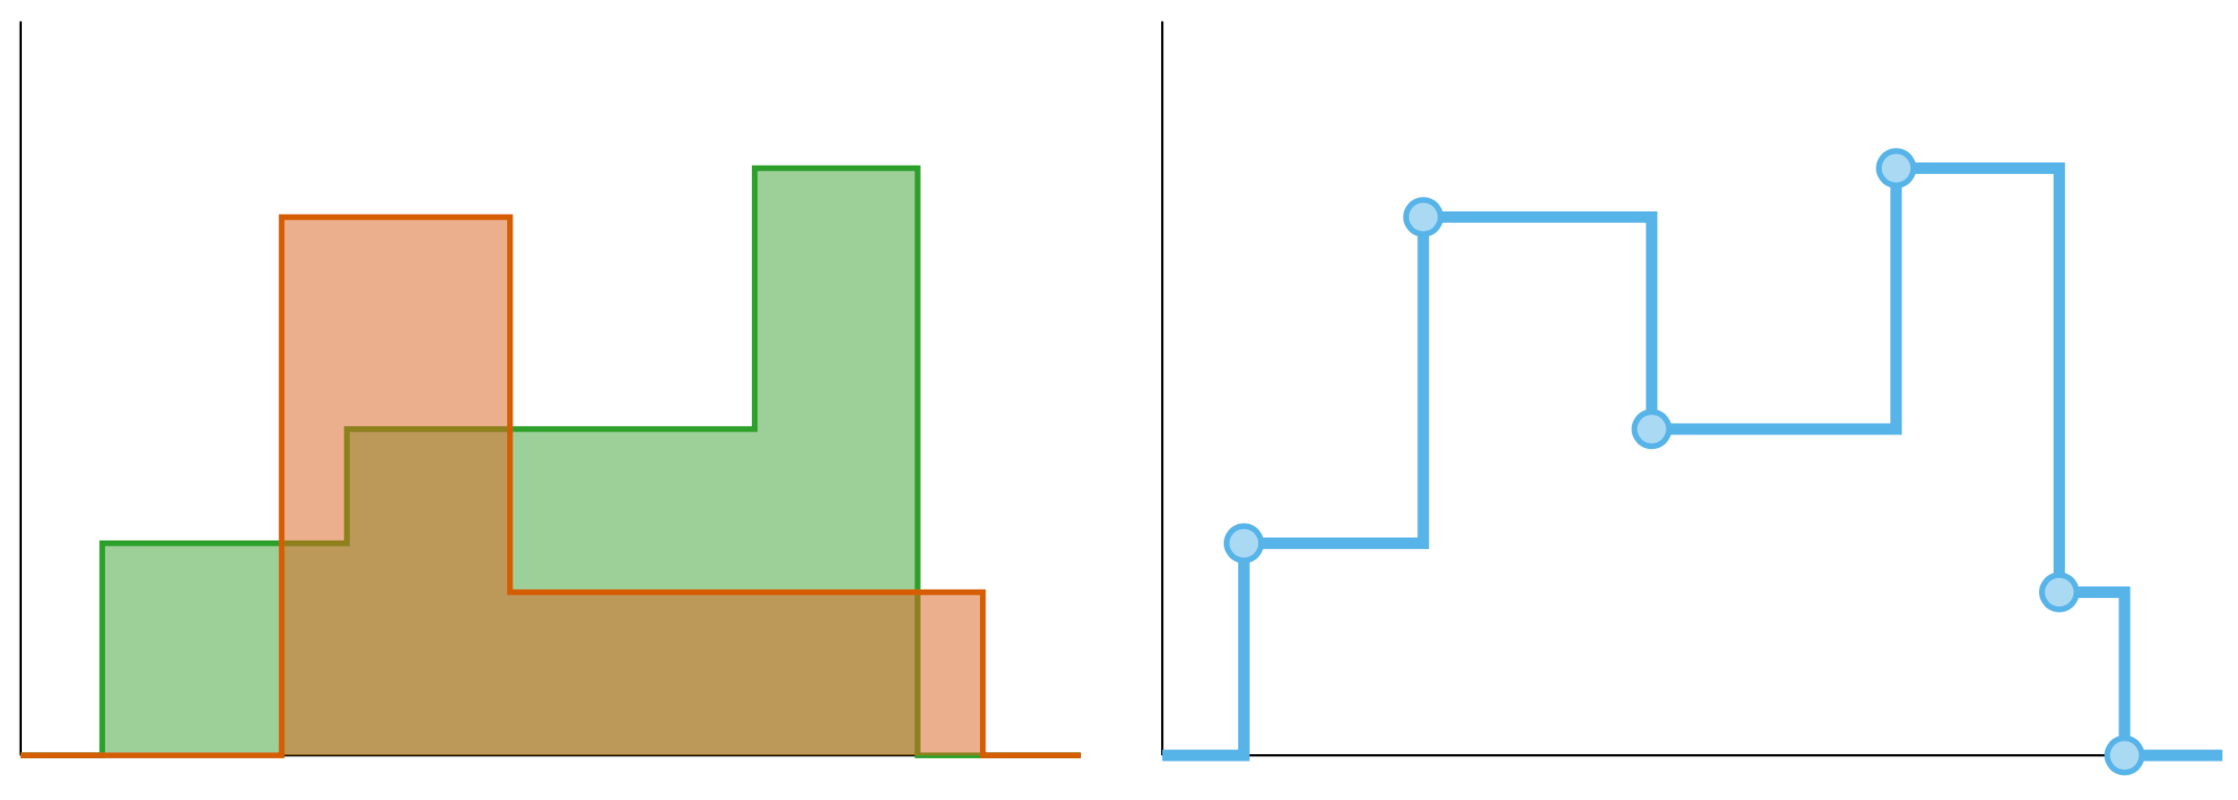
\includegraphics[width=0.8\textwidth]{../../Commun/Images/python-tp-horizon-3}\\
\textsc{Figure 3} -- Fusion de deux lignes d'horizon.
\end{center}
\question Écrire une fonction \verb!ligne_horizon1(bat: list[tuple[int, int, int]]) -> list[tuple[int, int]]!
  qui renvoie la ligne d'horizon associée aux bâtiments \verb!bat!, en partant d'une ligne d'horizon
  plate et en la fusionnant avec les lignes d'horizon des différents bâtiments. Quelle est sa complexité~?
\question En se basant sur la méthode \og diviser pour régner \fg, écrire une fonction
\begin{center}
  \verb!ligne_horizon2(bat: list[tuple[int, int, int]]) -> list[tuple[int, int]]!
\end{center}
  ayant les mêmes spécifications. Déterminer sa complexité.

\end{questions}


\section{Fonction $G$ de Hofstadter}
On définit la fonction $G$ de Hofstadter par
\[G(0)\defeq 0, \qquad\et\qquad \forall n\in\Ns\qsep G(n)\defeq n - G(G(n-1)).\]
\begin{questions}
\question Écrire une fonction récursive \verb!G(n: int) -> int! calculant $G(n)$.
\question Chronométrer le temps que votre ordinateur prend pour calculer $G(195)$.
\question Montrer par récurrence sur $n$ que quel que soit $n\in\N$, le calcul de $G(n)$ termine
  et $G(n)\leq n$.
\enonce Un problème posé par l'implémentation récursive de \verb!G! et qu'on se retrouve à calculer
  plusieurs fois de nombreux termes $G(k)$ lors du calcul de $G(n)$.
\question Écrire une fonction \verb!G_memoization(n: int) -> int!
  qui renvoie $G(n)$ mais qui évite de calculer plusieurs fois les différents $G(k)$. Cette fonction pourra
  utiliser un tableau d'entiers \verb!memo! de taille $n$ et remplir petit à petit les cases \verb!memo[k]!
  par $G(k)$.  Quel est le temps qui est désormais nécessaire pour calculer $G(195)$~?
\end{questions}
%END_BOOK
\end{document}